\documentclass{article}
\usepackage{fancyhdr} % for pretty formatting
\usepackage{amsmath} % for matrices
\usepackage{amssymb} % for bold text
\usepackage{pgfplots} % for graphs
\usepackage{hyperref} % for hyperlinks
\pgfplotsset{compat=1.18}

\usepackage{lipsum} % For dummy text
\usepackage{cite} % For citations

\pagestyle{fancy}
\fancyhf{} % Clear all header and footer fields

\lhead{Joshua Dunne}
\rhead{\thepage} % Displays the current page number
\lfoot{MATH620}
\rfoot{Unit 1}
\cfoot{Homework 2}

\begin{document}
    \section{Question 1}
        \subsection{Givens}
            \paragraph{Modes of transport}
                $\mathbf{v}_1=\begin{bmatrix}1\\1\\1\end{bmatrix}$
                $\mathbf{v}_2=\begin{bmatrix}6\\3\\8\end{bmatrix}$
                $\mathbf{v}_3=\begin{bmatrix}4\\1\\6\end{bmatrix}$
        \subsection{Questions}
            \renewcommand{\labelenumi}{\alph{enumi}}
            \begin{enumerate}
                \item
                    \begin{description} 
                        \item[Question:]Is there anywhere in $\mathbb{R}^3$ that old man Gauss can hide?
                        \item[Answer:]
                            Maybe, let's do a quick RREF and have a look
                            \[
                            \begin{bmatrix}
                            \begin{array}{ccc|c}
                                1 & 6 &  4 & x \\
                                0 & 3 &  8 & y \\
                                4 & 1 &  6 & z
                            \end{array}
                            \end{bmatrix}
                            \rightarrow
                            \begin{bmatrix}
                            \begin{array}{ccc|c}
                                1 & 0 & -2 & 0 \\
                                0 & 1 &  1 & 0 \\
                                0 & 0 &  0 & 1
                            \end{array}
                            \end{bmatrix}
                            \]
                            We're short a pivot in the bottom row but we do have an entry in the last column.
                            This means that the system is inconsistent and there is no solution.
                            So, there is somewhere in $\mathbb{R}^3$ that old man Gauss can hide.
                            We can also see that the vectors are linearly dependent.
                            \[
                            2\begin{bmatrix}1\\1\\1\end{bmatrix}
                            +
                            \begin{bmatrix}4\\1\\6\end{bmatrix}
                            =
                            \begin{bmatrix}6\\3\\8\end{bmatrix} 
                            =
                            \mathbf{v}_2
                            \]
                    \end{description}
            \end{enumerate}
    \section{Question 2}
        \subsection{Givens}
            \paragraph{Suppose}
                \[
                \mathbf{v_1}=\begin{bmatrix}1\\-1\\2\end{bmatrix}
                \mathbf{v_2}=\begin{bmatrix}-1\\2\\3\end{bmatrix}
                \mathbf{v_3}=\begin{bmatrix}2\\3\\h\end{bmatrix}
                \]
        \subsection{Question}
            \begin{description}
                \item[Question:]
                    For what values of $h$ are the vectors 
                    $\mathbf{v_1}$, $\mathbf{v_2}$, and $\mathbf{v_3}$ 
                    linearly dependent?
                \item[Answer:]
                    We can do this with the determinant this time around. The system
                    should result in a determinant that is $0$.
                    \[
                    det(
                        \begin{bmatrix}
                            1 & -1 & 2 \\
                            -1 & 2 & 3 \\
                            2 & 3 & h
                        \end{bmatrix}
                    )
                    =0
                    \]
                    \[
                    1(2h-9)+1(-h-6)+2(-3-4)=0
                    \]
                    \[
                    2h-9-h-6-6-8=0
                    \]
                    \[
                    h-29=0
                    \]
                    \[
                    h=29
                    \]
                \item[Check:]
                    So, given a value of $h=29$ we can check our work by calculating
                    \[
                    \mathbf{v_1}=\begin{bmatrix}1\\-1\\2\end{bmatrix}
                    \mathbf{v_2}=\begin{bmatrix}-1\\2\\3\end{bmatrix}
                    \mathbf{v_3}=\begin{bmatrix}2\\3\\29\end{bmatrix}
                    \]
                    \[
                    \begin{bmatrix}
                    \begin{array}{ccc|c}
                        1  & -1 & 2 & x \\
                        -1 & 2  & 3 & y \\
                        2  & 3  & 29 & z
                    \end{array}
                    \end{bmatrix}
                    \rightarrow
                    \begin{bmatrix}
                    \begin{array}{ccc|c}
                        1 & 0 & 7 & 0 \\
                        0 & 1 & 1 & 0 \\
                        0 & 0 & 0 & 1
                    \end{array}
                    \end{bmatrix}
                    \]
                    As we have a row of all zeros, we can be sure that the vectors are linearly dependent.

            \end{description}
    \section{Question 3}
        \subsection{Question}
            We're asked whether given $\{\mathbf{x}, \mathbf{y}\}$ as linearly independent.
            And given $\{\mathbf{x}, \mathbf{y}, \mathbf{z}\}$ as linearly dependent.
            Is $\mathbf{z}$ in the span of $\{\mathbf{x}, \mathbf{y}\}$?
            If false, give a counterexample.
        \subsection{Answer}
            Yes. For $\{\mathbf{x}, \mathbf{y}, \mathbf{z}\}$ to be linearly dependent,
            one of the vectors must be a linear combination of the others.
            That is, we could write $\mathbf{z}$ as $\mathbf{z} = a\mathbf{x} + b\mathbf{y}$
            for some $a$, $b \in \mathbb{R}$.
            This is another way of saying that $\mathbf{z}$ is in the span of $\{\mathbf{x}, \mathbf{y}\}$.
            So, if $\{\mathbf{x}, \mathbf{y}\}$ is linearly independent
            and $\{\mathbf{x}, \mathbf{y}, \mathbf{z}\}$ is linearly dependent,
            then $\mathbf{z}$ is in the span of $\{\mathbf{x}, \mathbf{y}\}$.
    \section{Question 4}
        \subsection{Remember from class}
            \begin{enumerate}
                \item 
                    If a set contains two vectors that are scalar
                    mulitples of one another, then the set 
                    is linearly dependent.
                \item 
                    If a set contains atleast two vectors that are
                    scalar multiples of one another, then the set is linearly dependent.
                \item    
                    If a set contains $p$ vectors in $\mathbb{R}^n$ 
                    and $p > n$
                    then the set is linearly dependent.
                \item
                    If a set contains the zero vector then it is linearly dependent.
                \item 
                    If a set contains exactly one vector, then the set is linearly independent
                    if and only if the vector is non-zero.
                \item 
                    A set of vectors is linearly dependent if and only if
                    one of the vectors can be expressed as a linear combination of the others.
            \end{enumerate}
        \subsection{Question}
            Choose two and write a reasonable explanation/proof.
        \subsection{Answers}
            \paragraph{Is a set containing two scalar multiples dependent?}
                Yes. If we have two vectors $\mathbf{v_1}$ and $\mathbf{v_2}$
                such that $\mathbf{v_2} = k\mathbf{v_1}$ for some $k \in \mathbb{R} \setminus \{0\}$.
                Then we can write
                \[
                k\mathbf{v_1} - \mathbf{v_2} = \mathbf{0}
                \]
                As we've expressed that atleast one vector is a scalar multiple
                of another, the set is linearly dependent.
            \paragraph{A set containing the zero vector is dependent?}
                Yes. If we have a set of vectors $\{\mathbf{v_1}, \mathbf{v_2}, \ldots, \mathbf{v_n}\}$
                and one of those vectors is the zero vector, say $\mathbf{v_1} = \mathbf{0}$.
                Then we can write
                \[
                1\cdot\mathbf{0} + 0\cdot\mathbf{v_2} + \ldots + 0\cdot\mathbf{v_n} = \mathbf{0}
                \]
                As we've expressed that one of the vectors is a linear combination
                of the others, the set is linearly dependent.
    \subsection{Question 5}
        Take a row from task 4 and describe the span of the vectors.
        \paragraph{A set of 2 vectors in $\mathbb{R}^3$}
            \subparagraph{Linearly Independent}
                \[
                \{
                    \begin{bmatrix}1\\1\\1\end{bmatrix}
                    \begin{bmatrix}2\\2\\2\end{bmatrix}
                \}
                \]
                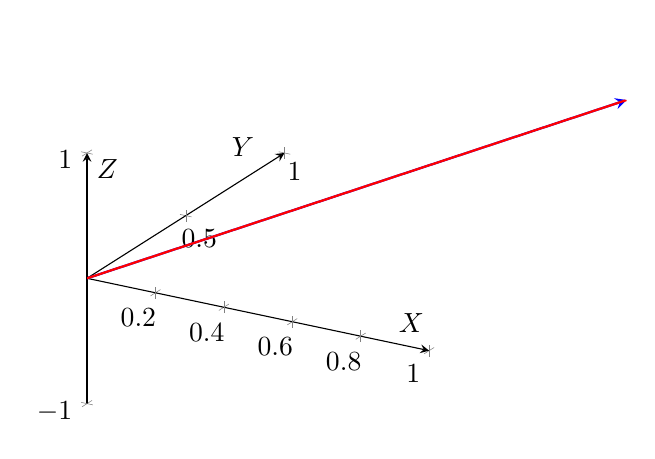
\begin{tikzpicture}
                    \begin{axis}[
                        xlabel=$X$,
                        ylabel=$Y$,
                        zlabel=$Z$,
                        grid=major,
                        axis lines=center, % Optional: center axes at origin
                        view={30}{30}, % Optional: set the viewing angle
                        zmin=-1, zmax=1
                    ]
                    \addplot3[
                        quiver={u=1,v=1,w=1},
                        -stealth,
                        thick,
                        color=blue
                    ] coordinates {(0,0,0)};
                    \addplot3[
                        quiver={u=2,v=2,w=2},
                        -stealth,
                        thick,
                        color=red
                    ] coordinates {(0,0,0)};
                        % Plot commands go here
                    \end{axis}
                \end{tikzpicture}
                We can see from abovec that the two columns are
                coincident. This means that the span of these two vectors
                is a line in $\mathbb{R}^3$.
                \[\mathbf{v}_2 = k\mathbf{v}_1 = 2\mathbf{v}_1\]
                Taking either from the pairing would give us the same line.
            \subparagraph{Linearly Dependent}
                \[
                    \begin{bmatrix}1\\0\\0\end{bmatrix}
                    \begin{bmatrix}0\\1\\0\end{bmatrix}
                \]
                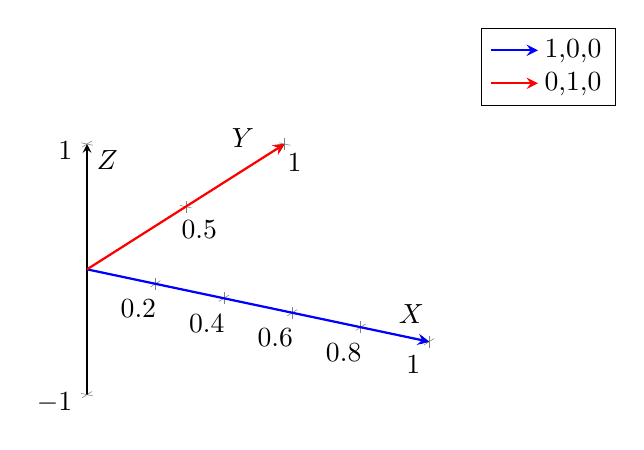
\begin{tikzpicture}
                    \begin{axis}[
                        xlabel=$X$,
                        ylabel=$Y$,
                        zlabel=$Z$,
                        grid=major,
                        axis lines=center, % Optional: center axes at origin
                        view={30}{30} % Optional: set the viewing angle
                    ]
                    legend style={at={(1,1)},anchor=south east},
                    \addplot3[
                        quiver={u=1,v=0,w=0},
                        -stealth,
                        thick,
                        color=blue
                    ] coordinates {(0,0,0)};
                    \addlegendentry{1,0,0}
                    \addplot3[
                        quiver={u=0,v=1,w=0},
                        -stealth,
                        thick,
                        color=red
                    ] coordinates {(0,0,0)};
                    \addlegendentry{0,1,0}
                        % Plot commands go here
                    \end{axis}
                \end{tikzpicture}
                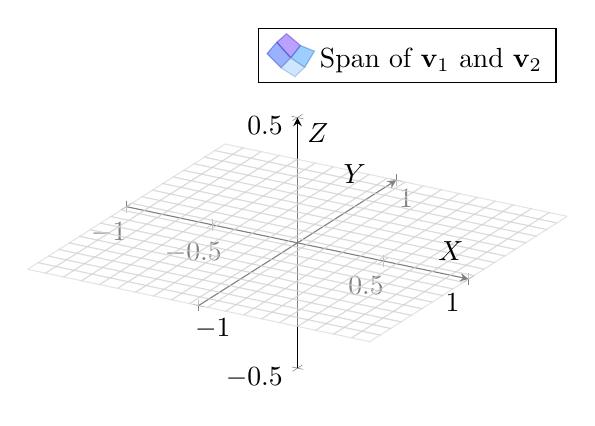
\begin{tikzpicture} %now to show the plane those span
                    \begin{axis}[
                        xlabel=$X$,
                        ylabel=$Y$,
                        zlabel=$Z$,
                        grid=major,
                        axis lines=center, % Optional: center axes at origin
                        view={30}{30}, % Optional: set the viewing angle
                        colormap/cool, % Choose a colormap
                        domain=-1:1, % Set the domain for x and y
                        y domain=-1:1, % Set the domain for y
                        samples=20, % Number of samples in each direction
                        samples y=20, % Number of samples in y direction
                        zmin=-0.5, % Set minimum z value
                        zmax=0.5,  % Set maximum z value
                    ]
                    \addplot3[
                        surf,
                        opacity=0.5, % Adjust transparency
                    ]
                    {0}; % Plane equation z = 0
                    \addlegendentry{Span of $\mathbf{v}_1$ and $\mathbf{v}_2$}
                    \end{axis}
                \end{tikzpicture}
                So, as we are able to provide coefficients
                to each of either vector to reach any point
                for $x, y \in \mathbb{R}^2$ and $z=0$,
                We have no control over $z$.
\end{document}